\documentclass[letterpaper, 11pt]{article}

\usepackage[pdftex]{graphicx}
\usepackage{epstopdf}
\DeclareGraphicsRule{*}{mps}{*}{} 

\usepackage{amsmath, amsthm, amssymb}
\usepackage{listings}
\usepackage{float}
\usepackage{enumerate}
% \usepackage{mystyle}
\usepackage{hyperref}
\usepackage{tikz}
\usepackage{fancyheadings}
\usepackage{tensor}
\usepackage{mathrsfs}
\usetikzlibrary{positioning}
\usetikzlibrary{decorations.pathmorphing}
\usetikzlibrary{arrows}
\usetikzlibrary{decorations.markings}
%\usepackage{fullpage}
\usepackage[left=0.75in, top=1.25in, right=0.75in, bottom=1.25in]{geometry}
\newcommand{\lambdabar}{{\mkern0.75mu\mathchar '26\mkern -9.75mu\lambda}}

\numberwithin{equation}{section}
\numberwithin{figure}{section}

\begin{document}

\title{Plasma Physics}
\author{Matthew Kunz}
\date{July 18, 2016}

\maketitle

\section{Lecture 1 - Magnetohydrodynamics (MHD)}
\label{sec:lec1}

The officially provided notes is at \href{https://pitp.ias.edu/sites/pitp/files/kunz_1.pdf}{here}.

\begin{table}[h]
  \centering
  \begin{tabular}{|c|c|c|c|c|}
    \hline
    & SW ($1\,\mathrm{au}$) & ICM  ($\sim 100\,\mathrm{kpc}$) & GC ($0.1\,\mathrm{pc}$) & ISM (warm) \\ \hline
    $T$ & $10\,\mathrm{eV}$ & $8\,\mathrm{keV}$ & $2\,\mathrm{keV}$ & $1\,\mathrm{eV}$ \\ \hline
    $n$ & $10\,\mathrm{cm^{-3}}$& $5\times 10^{-3}\,\mathrm{cm^{-3}}$& $100\,\mathrm{cm^{-3}}$ & $1\,\mathrm{cm^{-3}}$ \\ \hline
    $B$ & $100\,\mathrm{\mu G}$ & $1\,\mathrm{\mu G}$ & $1\,\mathrm{mG}$ & $5\,\mathrm{\mu G}$ \\ \hline
    $v_{th,i}$ & $40\,\mathrm{km/s}$ & $1000\,\mathrm{km/s}$ & $600\,\mathrm{km/s}$ &  $10\,\mathrm{km/s}$ \\ \hline
    $v_{A}$ & $70\,\mathrm{km/s}$ & $30\,\mathrm{km/s}$ & $200\,\mathrm{km/s}$ & $10\,\mathrm{km/s}$ \\ \hline
    $\beta_i = v_{th,i}^2/v_A^2$ & $\sim 0.3-1$ & $\sim 10^3$ & $\sim 100$ & $\sim 1$ \\ \hline
    $\lambda_{mfp}$ & $\sim 0.1 - 1\,\mathrm{au}$ & $\sim 0.1 - 10\,\mathrm{kpc}$ & $\sim 0.01\,\mathrm{pc}$& $\sim 10^{-7}\,\mathrm{pc}$ \\ \hline
    $\rho_i$ & $\sim 10^{-7}\,\mathrm{au}$ & $\sim 1\,\mathrm{npc}$ & $\sim 1\,\mathrm{ppc}$ & $\sim 10^{-11}\,\mathrm{pc}$ \\ \hline
  \end{tabular}
  \caption{Scales}
  \label{tab:scales}
\end{table}

You can't teach MHD in 1.5 hours, so we will just highlight something useful to
most of us. The first thing we consider is what is called a Plasma. This is a
difficult question to answer. Many different people identify themselves as
plasma physicists. The above table is everything that can come into the umbrella
of plasma physics. Below is a diagram (from the notes) that encompasses 35
orders of magnitudes in scale:

\begin{figure}[h]
  \centering
  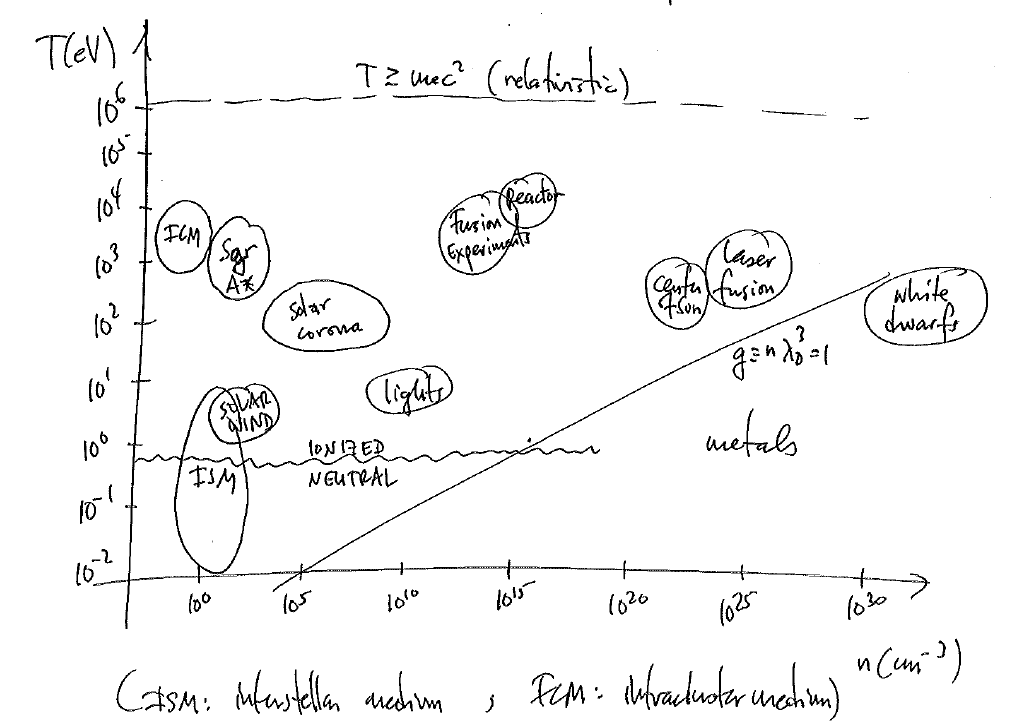
\includegraphics[width=0.8\textwidth]{scales.png}
  \caption{Scales of plasma physics}
  \label{fig:plasma}
\end{figure}

The one thing that is important is the line on the graph, which is the plasma
parameter which is defined as:
\begin{equation}
  \label{eq:1}
  g = n\lambda_D^3 = 1
\end{equation}
where $\lambda_D$ is the Debye length that is defined by the screening of the
charge in a plasma where
\begin{equation}
  \label{eq:1}
  \phi \sim \frac{1}{r}e^{-r/\lambda_D}
\end{equation}

The plasma parameter can be defined in various ways, and when we can treat
plasma as having collective behavior when $g \gg 1$:
\begin{equation}
  \label{eq:2}
  g \sim \frac{\text{KE}}{\text{PE}} \sim \frac{T}{e/\lambda_D} \sim \frac{\lambda_{mfp}}{\lambda_D} \gg 1
\end{equation}

In the table these are basically things that are interesting to us. SW refer to
the solar wind, which we can measure with spacecrafts. Other interesting media
we will see in following lectures are ICM (Inter-galactic medium), GC (Galactic
center), and ISM (Inter-stellar medium). The nice thing about the ISM is that
everything is about 1.

To get an idea of what the units mean, the Earth magnetic field is about
$0.5\,\mathrm{G}$. The thermal speed $v_{th,i}$ is a measure of the random
motion of particles
\begin{equation}
  \label{eq:3}
  v_{th,i} = \left( \frac{2T}{m_i} \right)^{1/2},\quad f \sim e^{-v^2/v_{th}^{2}}
\end{equation}

One more speed which is the Alfven speed
\begin{equation}
  \label{eq:4}
  v_A = \frac{B}{\sqrt{4\pi mn}}
\end{equation}
This is the speed that a disturbance propagates along the magnetic field. The
beta parameter $\beta_i$ is the ratio of the two velocities.

Now that we have defined what is a plasma, we need to talk about what is a
fluid. This is where the mean free path comes in $\lambda_{mfp}\sim
v_{th}\tau_\mathrm{col}$. This characterizes how often the particles scatter.
When this path is small like ISM the medium behaves like a fluid because the
distribution function looks very much like a Maxwellian. The larger this scale
gets you start to question whether this medium behaves like a fluid.

The last length scale is called $\rho_i$ which is $v_{th,i} / \Omega_i$ which is
the thermal speed divided by the gyro-frequency of the ion. This is the size of
a particle's gyration in a magnetic field. This scale is tiny compared to
most of other scales, which is characteristic of astrophysical plasmas. This
means the particles know about the magnetic field.

One more thing is the typical gyro-frequencies of particles. The table gives a
nice impression of the separation of scales for astrophysical situations. In a
typical plasma we should have $\lambda_\mathrm{Debye} \ll \rho_i \ll \lambda_{mfp}$

Now we will just write down the equations for plasma. Lets fix some notations
first. $\varrho$ is different from $\rho$, where the later means charge density,
and former means $\Sigma_sm_sn_s$.

The MHD equations
\begin{align}
  \frac{\partial\varrho}{\partial t} + \nabla\cdot(\varrho \mathbf{u}) &= 0 \\
  \frac{dM}{dt} = -\int \nabla\cdot(\varrho \mathbf{u})\,dV &= -\oint \varrho \mathrm{u}\cdot d\mathbf{S} \\
  \varrho \left( \frac{\partial \mathbf{u}}{\partial t} + \mathbf{u}\cdot \nabla \mathbf{u} \right) = -\nabla P + \mathbf{g}\varrho + \frac{\mathbf{J}\times\mathbf{B}}{c}
\end{align}
The third equation is basically Newton's second law. The left hand side is the
comoving derivative which we can also write as $D \mathbf{u}/Dt$. The third term
in the rhs is what makes MHD MHD, because we have Lorentz force. This is
implicitly non-relativistic, $v/c\ll 1$.

Lets talk a bit about the Lorentz force. We can rewrite it as
\begin{equation}
  \label{eq:5}
  \frac{\mathbf{J}\times \mathbf{B}}{c} = \frac{(\nabla\times \mathbf{B}) \times \mathbf{B}}{4\pi} = \frac{\mathbf{B}\cdot \nabla\cdot \mathbf{B}}{4\pi} - \nabla \frac{B^2}{8\pi}
\end{equation}
the second term is like a pressure of the magnetic field.

One last equation we want to write down is the entropy equation
\begin{equation}
  \label{eq:6}
  \frac{Ds}{Dt} = \frac{P}{\gamma - 1}\frac{D \ln P e^{-\gamma}}{D t} = \dot{Q}
\end{equation}
If we have a incompressible fluid $\nabla\cdot \mathbf{u} = 0$ then it implies
$T = \text{const}$ in a fluid element.

One difficulty of the MHD arises from the vector derivative $\mathbf{u}\cdot
\nabla \mathbf{u}$. It is very easy to drop terms when doing vector analysis. In
cylindrical coordinates for example, when we decompose the terms we will get the
Coriolis force and the centrifugal force. The details are sketched in the notes.

Now we have Maxwell equations:
\begin{align}
  \nabla\cdot \mathbf{B} & = 0 \\
  \frac{\partial \mathbf{B}}{\partial t} &= -c\nabla\times \mathbf{E} = \nabla \times (\mathbf{u}\times \mathbf{B}) - \nabla\times(\eta \nabla\times \mathbf{B})
\end{align}
the last term is a way to abstract the electric field where we could take
$\mathbf{E} = \eta \mathbf{J}$, which is just Ohm's law. The last term is a way
to characterize resistive diffusion in the fluid. This term is not important
when the magnetic Reynolds number is high.

The first term can be expanded using vector analysis
\begin{equation}
  \label{eq:7}
  \frac{\partial \mathbf{B}}{\partial t} = \mathbf{B}\cdot \nabla \mathbf{u} - \mathbf{u}\cdot \nabla \mathbf{B} - \mathbf{B}\nabla\cdot \mathbf{u}
\end{equation}
There is also a last term but it is zero because $\nabla\cdot \mathbf{B} = 0$.
The first term is called ``stretching'', the second ``advection'', and the third
``compression''.

One thing we can do is take this form of the induction equation, and the
continuity equation and combine them. We then have
\begin{equation}
  \label{eq:8}
  \frac{D}{Dt}\frac{\mathbf{B}}{\varrho} = \frac{\mathbf{B}}{\varrho}\cdot \nabla \mathbf{u}
\end{equation}
This means that if we have a point $\mathbf{x}$ moving with velocity
$\mathbf{u}$, and another point $\mathbf{x} + \boldsymbol{\xi}$ moving with
$\mathbf{u}(\mathbf{x} + \boldsymbol{\xi})$ then we have
\begin{equation}
  \label{eq:9}
  \frac{D\boldsymbol{\xi}}{D t} \approx \boldsymbol{\xi}\cdot \nabla \mathbf{u}
\end{equation}
What this means is that fluid elements that lie on field lines initially will
remain on the field lines. This is called the Lindquist theorem, or ``flux freezing''.

We also have the Alfven theorem which states that, if we have some surface $S$
and there are some magnetic field lines that threads the surface with $\Phi =
\int \mathbf{B}\cdot d\mathbf{S}$. If the above equation is true then the flux
does not change with the flow of the fluid: $d\Phi/dt = 0$. The magnetic field
is ``frozen'' into the fluid and if the fluid moves, the lines moves with it.

Now lets come back to the Lorentz force. Remember we have
\begin{equation}
  \label{eq:10}
  \frac{\mathbf{J}\times \mathbf{B}}{c} = \frac{\mathbf{B}\cdot \nabla \mathbf{B}}{4\pi} - \nabla \frac{B^2}{8\pi} = -\nabla\cdot \left[ \frac{B^2}{8\pi}\mathbf{I} - \frac{\mathbf{B} \mathbf{B}}{4\pi} \right] = -\nabla \mathbf{M}
\end{equation}
where $\mathbf{M}$ is called the Maxwell stress tensor. The first term in the
bracket is diagonal, and the second term is the thing that introduces anisotropy
to the system by Lorentz force.

People usually say the first term is pressure and second term is tension but
that is not exactly true. Lets define $\hat{b} = \mathbf{B}/B$. We can write
the Lorentz force as
\begin{equation}
  \label{eq:11}
  \mathbf{F} = \frac{B^2}{4\pi} \hat{b}\cdot\nabla \hat{b} - (\mathbf{I} - \hat{b} \hat{b})\cdot \nabla \frac{B^2}{8\pi}
\end{equation}
The first term is apparently perpendicular to the field line, and can be thought
of as the curvature force, as in the curved field line wants to be straightened.
The second term creates pressure towards the region where magnetic field is
small, wanting to spread out the field lines to be more even. This Lorentz force
is the fundamental difference between MHD and hydro, because magnetic field
doesn't want to be messed with, and it will direct the fluid.

An important part of MHD is the linear theory. We expand the quantities we are
interested in around an ``equilibrium'':
\begin{equation}
  \label{eq:12}
  \mathbf{u} = \mathbf{u}_0 + \delta \mathbf{u},\quad \varrho = \varrho_0 + \delta\varrho,\quad
  \mathbf{B} = \mathbf{B}_0 + \delta \mathbf{B},\quad P = P_0 + \delta P
\end{equation}
we use $\delta$ to denote Eulerian perturbation, and $\Delta$ to be Lagrangian
perturbation, where the former means the perturbation in lab frame, and the
latter means a change in the comoving frame of the fluid. Lets use Eulerian
perturbations for now for simplicity.

We have some equilibrium state denoted by suffix zero, and introduce some
perturbation to it, and in linear theory we just drop all the quadratic terms in
perturbation: $\delta^2 \longrightarrow 0$. In a homogeneous stationary plasma,
after we drop the quadratic terms we replace the perturbation with
\begin{equation}
  \label{eq:13}
  \delta \sim e^{-i\omega t + i\mathbf{k}\cdot \mathbf{r}}
\end{equation}
and then just do linear algebra.

One thing we can get out of this is called the Alfven wave. This is when
$\mathbf{k} = k_{\parallel}\hat{b}_0$. There is no change in $B_{\parallel}$ and
$\varrho$. The dispersion relation is very simple
\begin{equation}
  \label{eq:14}
  \omega = \pm k_{\parallel}v_A
\end{equation}
This is the fundamental building block of plasma perturbations.

We can also have compression waves in the fluid, which is like sound wave
\begin{equation}
  \label{eq:15}
  \omega = \pm k_{\parallel}c_s,\quad c_s = \left( \frac{\gamma P_0}{\varrho_{0}} \right)^{1/2}
\end{equation}
where $c_s$ is the speed of sound in the fluid.

We can also have a whole class of magnetic-sonic waves. Let $\mathbf{k} =
k_{\parallel}\hat{b}_0 + \mathbf{k}_{\perp}$. In regions with high $P$ and high
$B$, we have fast wave, and in regions with small $B$ we have slow wave. The
details of these waves are in the notes.

There is also an entropy mode where $\omega = 0$. That is all the mode we want
to talk about in MHD.

There is one more section which is called the Reduced MHD, but we are going to
skip it because of time. It is a useful technique for doing asymptotic
expansions.

When we wrote down all the equations we didn't talk about what was the velocity.
In MHD it is technically defined as
\begin{equation}
  \label{eq:16}
  \mathbf{u} = \frac{\sum_sm_sn_s\mathbf{u}_s}{\sum_sm_sn_s}
\end{equation}
which basically means center-of-mass velocity. In the limit of $n_i/n_n \ll 1$
the fluid velocity is governed by the neutral particle velocity which may not
make sense in MHD because neutral particles are not coupled to the magnetic
field. That is why we need to talk about multi-fluid MHD.

If we derive everything from the Vlasov equation, we can see that we have
continuity equation for every species
\begin{equation}
  \label{eq:17}
  \frac{\partial n_s}{\partial t} + \nabla\cdot \left( n_s\mathbf{u}_s \right) = 0
\end{equation}
and force equation for every species
\begin{equation}
  \label{eq:18}
  m_sn_s\frac{D \mathbf{u}_s}{D t_s} = -\nabla P_s + q_sn_s \left( \mathbf{E} + \frac{\mathbf{u}_s\times \mathbf{B}}{c} \right) + \mathbf{R}_s
\end{equation}
where the last term is the friction between species which add up to zero when we
sum all species. We also have the entropy equation for each species.

When we write down the induction equation for multi-fluid plasma, what should we
use as the plasma velocity $\mathbf{u}$? Suppose there is some frame where the
magnetic field is frozen, such that
\begin{equation}
  \label{eq:19}
  \frac{\partial \mathbf{B}}{\partial t} = \nabla \times \left( \mathbf{u}_f\times \mathbf{B} \right)
\end{equation}
for some $\mathbf{u}_{f}$. We can write it as
\begin{equation}
  \label{eq:20}
  \frac{\partial \mathbf{B}}{\partial t} = \nabla \times \left[ (\mathbf{u}_f - \mathbf{u}_{e}) \times \mathbf{B} + (\mathbf{u}_{e} - \mathbf{u}_{i})\times \mathbf{B} + (\mathbf{u}_{i} - \mathbf{u}_{n})\times \mathbf{B} + u_n\times \mathbf{B} \right]
\end{equation}
The three terms can be associated with different things. $u_f - u_{e}$ is what
we call Ohmic dissipation, which is like collisional resistivity. $u_i - u_n$ is
associated with Ambipolar diffusion, and $u_{i} - u_{e}$ is associated with Hall
effect. The Hall effect is related to nothing but the current $\mathbf{J} =
en_i(\mathbf{u}_{i} - \mathbf{u}_{e})$. Because $\mathbf{J} = \nabla\times
\mathbf{B}$ this introduces wave dispersion in MHD.

Lets come back to ambipolar diffusion. When do we expect $u_i$ and $u_n$ to
differ? This is related to the collision time scale between ions and neutral
particles
\begin{equation}
  \label{eq:21}
  \frac{u_i - u_n}{\tau_{ni}} \sim \frac{1}{\varrho_n}\left( \frac{\mathbf{J}\times \mathbf{B}}{c} \right)
\end{equation}
This is a kind of anisotropic diffusion for the magnetic field. It is useful to
re-derive the linear theory with these kind of drift speed between different
species of particles, and see what happens to different kinds of waves.

Where can we use these MHD? In solar wind people have used reduced MHD but
that's about it, because solar wind the fluid is not very collisional. In ICM
the collision is not quite strong enough. In GC the mean free path is about the
Bondi radius, especially if we keep going in near the black hole it is worse.
ISM has a cold and a warm phase, but both are pretty good for MHD.

\section{Lecture 2 - Kinetics}
\label{sec:lec2}

Lets start with a recap. MHD is a fluid theory, where $\lambda_\mathrm{Debye}$
is infinitesimal, meaning the fluid is quasi neutral. Another thing is that the
ion gyro path is infinitesimal. The third quantity is the mean free path which
is infinitesimal. MHD is a fluid theory of infinitesimal fluid elements subject
to the Lorentz force.

What if we want to relax some of the above assumptions? Suppose we are dealing
with ICM, SW, GC, etc.\ which are not in the ideal MHD regime. There are a
number of different ways to relax the assumptions:
\begin{itemize}
    \item Tracing particle motion, guiding center motion. Most of the kinetic
      discussions start with particle motion.
    \item Adiabatic invariance, pressure anisotropy. Deviations from Maxwell distribution.
    \item Braginskii-MHD and ``CGL'' equations (monograph from 1965).
    \item What if collisions are not strong enough? We need to give up MHD as a theory:
    \item Vlasov-Landau kinetic equation. Dealing with distribution functions directly.
    \item Ordering parameters. For the system of interest, what are the small
      parameters so that we can expand our system of equations in terms of these
      small parameters?
    \item Kinetic MHD:\@Barnes \& Landau damping, Firehose \& mirror instabilities.
    \item Preview of gyrokinetics. This is an advanced tool that astrophysics
      should pick up in their toolset. A simple derivation is in the notes.
\end{itemize}

\subsection{Particle Motion}

There are two types of particle motion in EM field. If we have a particle at
position $\mathbf{r}$, which is gyrating along some $\mathbf{B}$ field. It makes
a lot of sense to define another vector $\mathbf{R}$ which is the center of the
Larmor motion of the particle. The motion of the particle can be decomposed into
the motion of the guiding center and the gyration itself. Let $\mathbf{r} =
\mathbf{R} + \mathbf{\rho}$. We have
\begin{equation}
  \label{eq:22}
  \mathbf{\rho} = -\frac{\mathbf{v}\times \hat{b}}{\Omega}, \quad \hat{b} = \frac{\mathbf{B}}{B},\quad \Omega = \frac{qB}{mc}
\end{equation}

If $B$ and $E$ are uniform and time independent, we can easily write down how
the guiding center evolves
\begin{equation}
  \label{eq:23}
  \begin{split}
    \dot{\mathbf{R}} &= \dot{\mathbf{r}} - \dot{\rho} \\
    &= \mathbf{v} + \frac{q}{m}\left[ \mathbf{E} + \frac{\mathbf{v}\times \mathbf{B}}{c} \right]\times\frac{\hat{b}}{\Omega} \\
    &= v_{\parallel}\hat{b} + c\frac{\mathbf{E} \times \mathbf{B}}{B^2}
  \end{split}
\end{equation}
The second term is called the ``E cross B'' drift. To get an idea of what it
does, consider a particle in a $B$ field which simply gyrates in a circle. If we
add $E$ field to the system. We know that $\rho = v_{\perp}/\Omega$. As particle
gyrates it gets accelerated so $\rho$ increases, but when it comes back it
decelerates. So on average its gyration is drifting in the $\mathbf{E}\times
\mathbf{B}$ direction.

The important thing about this drift is that it is species-independent. This
means that this drift introduces no current. For general force $\mathbf{F} \neq
q\mathbf{E}$, we can generalize the formula for the drift to be
\begin{equation}
  \label{eq:24}
  \dot{\mathbf{R}}_\mathrm{dirft} = \frac{c \mathbf{F}\times \mathbf{B}}{qB^2}
\end{equation}

Now lets make the magnetic field non-uniform but still static. Lets repeat the
whole calculation. The total derivative is with respect to the particle
trajectory $d/dt \to \partial/\partial t + \mathbf{v}\cdot\nabla$
\begin{equation}
  \label{eq:25}
  \begin{split}
    \dot{\mathbf{R}} &= \dot{\mathbf{r}} - \dot{\rho} \\
    &= v_{\parallel}\hat{b} + \frac{c \mathbf{E}\times \mathbf{B}}{B^2} + \mathbf{v}\times \frac{d}{dt}\left( \frac{\hat{b}}{\Omega} \right)
  \end{split}
\end{equation}
The last term is new. It will give two things: grad-B drift and the curvature
drift. From the mathematics view it is just vector calculus, but we can reason
it from the physics point of view. We associate a force to when $B$ is
non-uniform, and a force to when $B$ has some curvature. When $B$ is not
uniform, remember
\begin{equation}
  \label{eq:26}
  \mathbf{F} = \nabla \left( \mu \cdot \mathbf{B} \right), \quad \mu = -\frac{1}{2}\frac{mv_{\perp}^2}{B}\hat{b}
\end{equation}
If we put this into the formula we get
\begin{equation}
  \label{eq:27}
  \hat{\mathbf{v}}_{\nabla B} = \frac{v_{\perp}^2}{2\Omega}\hat{b}\times \nabla \ln \mathbf{B}
\end{equation}
This means that the particle drifts perpendicular to the direction where there
is gradient of $B$. The curvature drift is similar with
\begin{equation}
  \label{eq:28}
  \hat{\mathbf{v}}_\mathrm{curv} = \frac{m v_{\perp}^2}{r_{c}}\hat{r}_{c}
\end{equation}

\subsection{Adiabatic Invariance}

In plasma physics adiabatic invariance is associated with some periodic motion
that particles undergo. One kind of such motion is simply the gyration around $B$
fields. Another kind of periodic motion is associated with the drifts, for
example a particle bouncing in a magnetic bottle. We will now talk about this
kind of motion in detail. This is similar to the Poincare invariant in
kinematics $I = \oint \mathbf{p}\cdot d\mathbf{q}$.

We wrote down the magnetic moment of the particle $\mu = mv_{\perp}^2/2B$. This
is actually the first adiabatic invariant. If for example a particle is gyrating
in a uniform $B$ field, and we very slowly decrease the magnetic field. We can
see that the perpendicular velocity of the particle will adjust and decrease as
well, so that this quantity is conserved. Another way to look at it is that
magnetic flux in the Larmor orbit is conserved.

One can show that $\mu$ is conserved to the precision of $e^{-\Omega/\omega}$
where $\omega$ is the rate of change of the magnetic field. We call this
conservation ``to all orders'' since it is exponential.

Another conserved quantity is $J = \oint m v_{\parallel} d\ell_B$ where $\ell_B$
is the path along $B$ and $v_{\parallel}$ is the guiding center motion parallel
to the magnetic field. Consider a magnetic bottle. Since energy of the particle
is conserved and also $\mu$ is conserved, so $v_{\parallel}^2$ will decrease in
regions of large $B$, and particles will eventually reflect. In this kind of
periodic mirroring motion, $J$ is conserved.

\subsection{Anisotropy}

If we look at the magnetic moment of a species of particles and take the
expectation value
\begin{equation}
  \label{eq:29}
  \left<\mu \right> = \frac{\int \mu f d^3V}{\int f d^3V} = \frac{\int \frac{1}{2}\frac{mv_{\perp}^2}{B}f d^3V}{n} = \frac{P_{\perp}}{nB} = \frac{T_{\perp}}{B}
\end{equation}

One can do the same thing with $J$:
\begin{equation}
  \label{eq:30}
  \left\langle J^2 \right\rangle = \frac{\int m^2v_{\parallel}^2\ell_B^2 f d^3V}{\int f d^3V} = \frac{T_{\parallel}B^2}{n^2}
\end{equation}
where we choose $\ell = B/n$. These are the two most important quantities when
one goes to weakly collisional systems. This means that if we adjust $B$ or $n$
then the perpendicular/parallel motion of the particles will collectively
adjust.

In terms of a fluid we can write this in a nicer way
\begin{equation}
  \label{eq:31}
  \frac{D}{Dt}\left( \frac{P_{\perp}}{nB} \right) \approx 0,\quad \frac{D}{Dt}\left( \frac{P_{\parallel}B^2}{n^3} \right) \approx 0
\end{equation}
These are called double adiabatic laws and replaces the equation of entropy. A
nice paper discussing this is \href{http://rspa.royalsocietypublishing.org/content/236/1204/112}{(Chew, Goldberger, \& Low 1956)}. The total $P$ can
be split such that $P = 2P_{\perp} / 3 + P_{\parallel} / 3$.

We now want to introduce a right hand side to these equations. We take the
difference of the equations we get
\begin{equation}
  \label{eq:32}
  \left[ \frac{D}{Dt} + \frac{D(\ln B n^{-7/3})}{Dt} \right](P_{\perp} - P_{\parallel}) = 3P \frac{D\ln B n^{-2/3}}{Dt} + \text{heat flows} + \text{cooling/heating} - \nu(P_{\perp} - P_{\parallel})
\end{equation}
This is one version of the so-called CGL equations.

One distribution function that exhibits this anisotropy is the ``bi-Maxwellian''
distribution
\begin{equation}
  \label{eq:33}
  \frac{f}{n} = \frac{e^{-v_{\perp}^2/v_{th\perp}^2} e^{-v_{\parallel}^2/v_{th\parallel}^2}}{\pi^{3/2}v_{th\perp}^2v_{th\parallel}}
\end{equation}

Consider the limit where the frequency of time changes $\omega \sim D/Dt \ll
\nu_\mathrm{coll} \ll \Omega$. This limit is good for ICM, GC, etc. The entire
left hand side of the above equation can be dropped, and the largest term is the
$\nu$ term on the right.

This limit is considered in \href{http://adsabs.harvard.edu/abs/1965RvPP....1..205B}{(Braginskii 1965)}. We can rewrite the equation as
\begin{equation}
  \label{eq:34}
  P_{\perp} - P_{\parallel} = \frac{3P}{\nu}\frac{D \ln}{Dt}\frac{B}{n^{2/3}} = \frac{3P}{\nu}\left( \hat{b}\hat{b} - \frac{1}{3}\mathbf{I} \right):\nabla \mathbf{u}
\end{equation}
where $\mathbf{a}\mathbf{b}:\nabla \mathbf{c} = a_ib_j\partial c_j/\partial x_i$.

Lets try to understand how this connects to our previous discussions. One way to
include this anisotropy in our fluid equations is to promote $P$ to a tensor:
\begin{equation}
  \label{eq:35}
  \mathbf{P} = P_{\perp}\left( \mathbf{I} - \hat{b}\hat{b} \right) + P_{\parallel}\hat{b}\hat{b}
\end{equation}
The equation can be closed because of our previous equation. This new pressure
term introduces anisotropy viscosity. It is also called the ``Braginskii
viscosity''.

What this equation says is that there is viscosity, but the viscosity only acts
along the magnetic field lines, because with the ordering it is incredibly
difficult to communicate between the field lines due to particles restrained to
gyrate around the field lines in very small orbits.

This is already very different from MHD, where the only anisotropy is due to the
Lorentz force. Now if there is heat flux in the system it is subject to the same
constraint of flowing along the magnetic field:
\begin{equation}
  \label{eq:36}
  \mathbf{Q} = -\chi \hat{b} \hat{b}\cdot\nabla T
\end{equation}
Notice the appearance of the tensor $\hat{b}\hat{b}$. This is called anisotropic
conduction.

\subsection{Collision Not Strong Enough}

We picked up the first order correction to MHD which is pressure anisotropy. Let
us now talk about when collision is not enough and we need to consider kinetics.
However kinetics is a very deep subject because one doubles the dimensions of
the problem by introducing distribution functions.

The kinetic equation is a statistical description of the plasma. The problem
about simulating a system of particles directly is that we have too many
particles ($\sim 10^{28}$). Another problem is that it is very sensitive to
initial conditions because particle trajectories are chaotic. The third problem
is that we are not interested in the individual particles but only some
collective quantities, so why trace them individually in the first place?

We instead describe a large number of particles using their collective
statistical properties which is their distribution in the phase space
\begin{align}
  \int f(t, \mathbf{x}, \mathbf{v})\,d^3v &= n \\
  \int f \mathbf{v}\,d^3v &= n \mathbf{u} \\
  \int f \frac{1}{2}m v_{\perp}^2\, d^{3}v &= P_{\perp}
\end{align}

The equation for the distribution function is
\begin{equation}
  \label{eq:37}
  \frac{df}{dt} = \frac{\partial f}{\partial t} + \mathbf{v}\cdot\nabla f + \mathbf{a}\cdot \frac{\partial f}{\partial \mathbf{v}} = C[f]
\end{equation}
This is called the Vlasov equation where the right hand side is a functional
describing the collisional terms. It has 3 spatial and 3 velocity dimensions, so
solving it is very expensive. In addition this is coupled to Maxwell equations,
which we need to solve simultaneously.

This equation is extremely rich, even when doing linear theory. What happens if
we don't want to solve this? We can remove some degrees of freedom, reduce
dimensions, or find other approximations. One way is to find small parameters
$\epsilon \ll 1$. One possible one is that $\epsilon \sim \omega/\Omega$,
meaning the rate of change is small compared to gyro frequency. It could be
$\epsilon \sim \rho/\ell$, $\epsilon \sim v/c$, etc. These are starting points
of kinetic MHD, and gyrokinetics. The simple derivations of these are in the
notes.

In kinetic MHD, we have $\rho/\ell \sim \epsilon$ where $\ell$ is any scale in
the problem. However in gyrokinetics we have $\rho/\rho_{\parallel}\sim
\epsilon$ but $\rho/\rho_{\perp}\sim 1$. This is an important distinction
between them.

\subsection{Instabilities}

We will briefly cover some instabilities. First one is the Firehose instability.
It is basically Alfven waves when
\begin{equation}
  \label{eq:38}
  P_{\parallel} > P_{\perp} + \frac{B^2}{4\pi}
\end{equation}
When this happens the magnetic field will develop wild oscillations.

Another is the Mirror instability which is associated with the growth of slow
modes. If we have a series of magnetic mirrors and if we squeeze the fields the
particles will move away from that point. When
\begin{equation}
  \label{eq:39}
  P_{\perp} > P_{\parallel} + \frac{B^2}{8\pi}
\end{equation}
the mirrors will grow and become unstable.




\end{document}
